\chapter{System Design}

\section{Introduction}
System design converts the requirements into a working architecture. The proposed system is designed as a client-server web application with a React frontend, Flask backend, SQLite database, and Gemini Vision model integration. The architecture separates user interaction, model inference, policy logic, action handling, and persistence.

\section{System Architecture Design}
The system architecture is shown in Fig. \ref{fig:systemarchitecture}. The frontend accepts image input and displays chat messages. The backend receives the request, validates input, sends the image to Gemini Vision, parses the response, applies normalization and risk rules, saves records, and returns action buttons to the frontend.

\begin{figure}[H]
\centering
\fbox{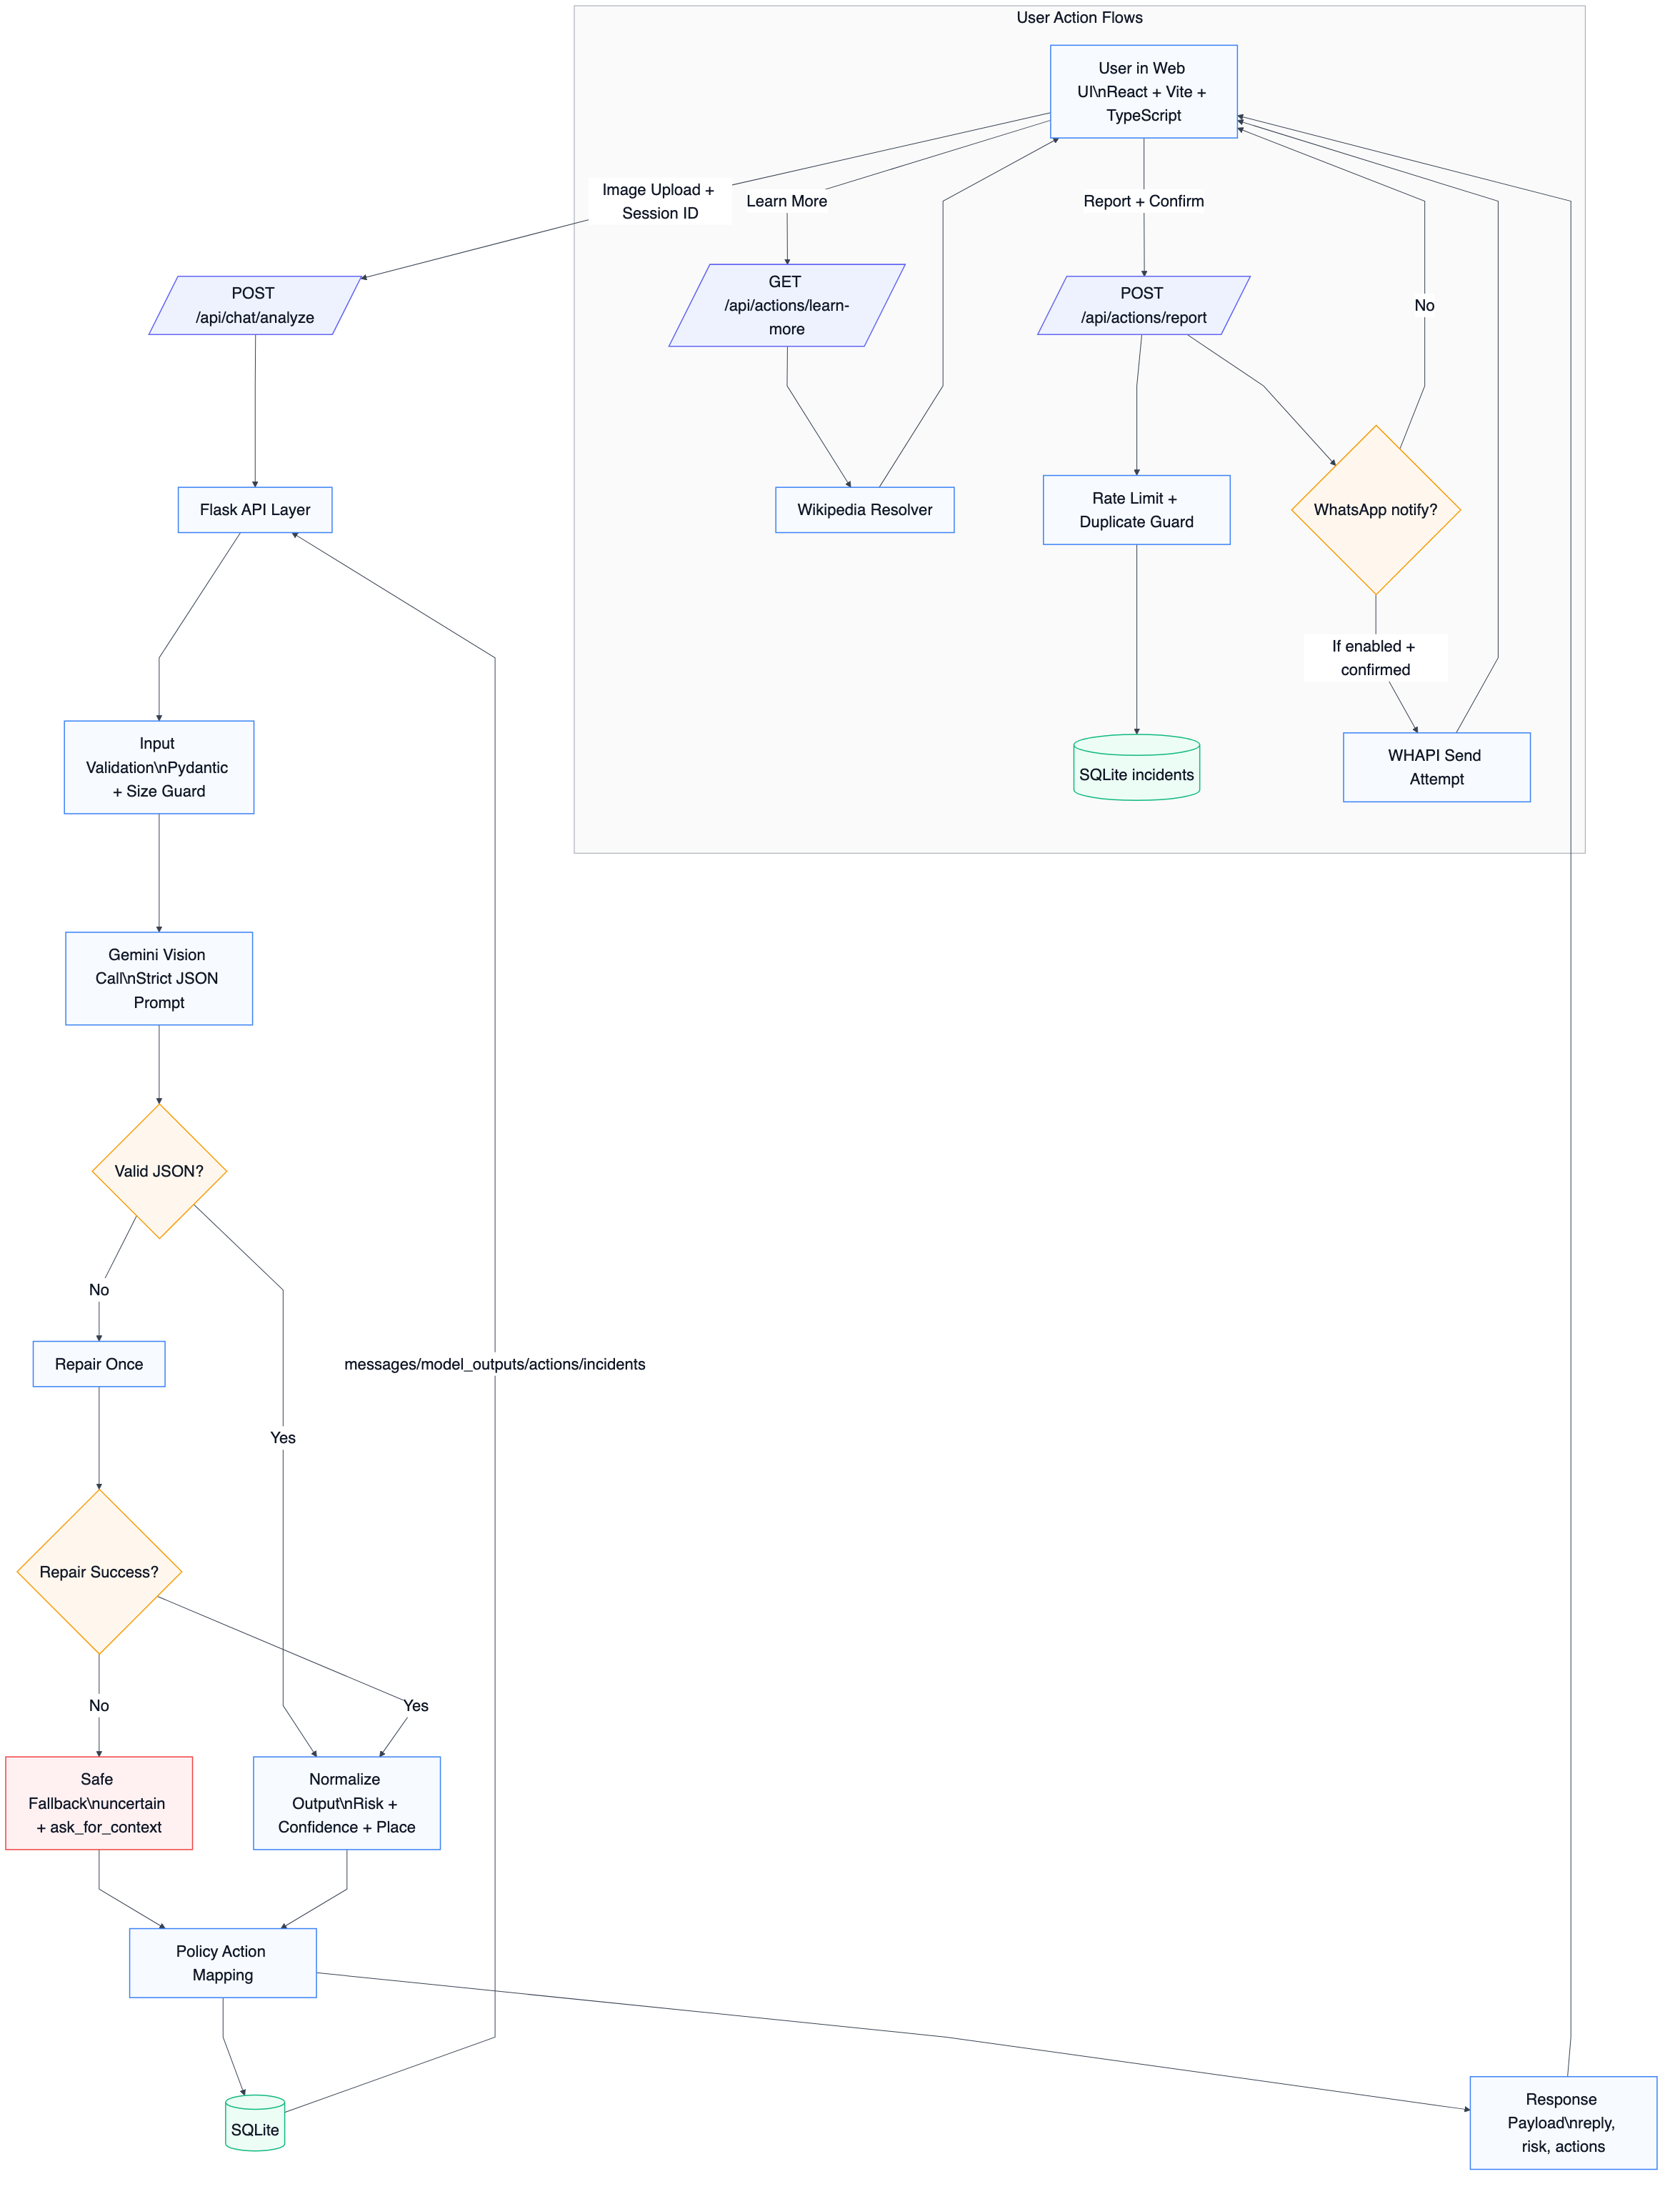
\includegraphics[width=0.95\textwidth]{../paper/figures/system_architecture.png}}
\caption{System architecture}
\label{fig:systemarchitecture}
\end{figure}

The main modules are:
\begin{itemize}
\item \textbf{User Interface}: Provides image upload, preview, chat timeline, and action buttons.
\item \textbf{Backend API}: Handles analyze, learn-more, report, and health endpoints.
\item \textbf{Multimodal Inference}: Sends image and prompt to Gemini Vision and requests strict JSON.
\item \textbf{Parser and Normalizer}: Extracts JSON, repairs invalid output once, validates fields, and normalizes confidence.
\item \textbf{Risk Policy}: Converts model output and hazard signals into final risk and confidence.
\item \textbf{Action Mapper}: Generates actions such as report, learn-more, open map, safety tips, and why.
\item \textbf{Persistence Layer}: Stores sessions, messages, model outputs, actions, and incidents in SQLite.
\end{itemize}

\section{Mathematical Model for the Proposed System}
Let the input image be represented by $I$ and optional user context be represented by $T$. The multimodal model produces a structured output:
\[
o = M(I,T)
\]
where $o$ contains summary, risk level, confidence, entities, possible location, rationale, and recommended actions.

Let $r_m$ be the model risk level and $c_m$ be the model confidence. Let $h=1$ if hazard keywords are present in the summary, rationale, user context, or location text; otherwise $h=0$. The final risk is:
\[
r =
\begin{cases}
\text{high}, & h=1 \text{ and } r_m \in \{\text{low, uncertain}\} \\
r_m, & \text{otherwise}
\end{cases}
\]

The confidence value is normalized to the range $[0,1]$. When a hazard signal is detected, the confidence is adjusted as:
\[
c = \max(c_m, 0.72) \quad \text{when } h=1
\]

The action set $A$ is selected using deterministic policy rules:
\[
A =
\begin{cases}
\{\text{ask\_for\_context}, \text{why}\}, & c < 0.45 \text{ or } r=\text{uncertain} \\
\{\text{report}, \text{safety\_tips}, \text{why}\}, & r=\text{high} \\
\{\text{safety\_tips}, \text{why}\}, & r=\text{medium} \\
\{\text{learn\_more}, \text{open\_map}, \text{why}\}, & r=\text{low}
\end{cases}
\]

\begin{algorithm}[H]
\caption{Hazard-Aware Image Analysis Flow}
\KwIn{Input image $I$ and optional message $T$}
\KwOut{Structured response and action set $A$}
Generate structured model output $o \leftarrow M(I,T)$\;
Extract JSON from model output\;
\If{JSON is invalid}{
Attempt one repair pass\;
}
\If{repair fails}{
Return safe fallback output\;
}
Normalize summary, risk, confidence, entities, and location\;
Detect hazard signal $h$\;
Apply risk and confidence policy\;
Generate action set $A$\;
Persist message, output, and action records\;
Return response to frontend\;
\end{algorithm}

\section{Data Design}
The internal data structure uses Python dictionaries and Pydantic models for API validation. The global data structure is the SQLite database. Temporary data includes uploaded image bytes, base64 encoded image content, parsed model JSON, and generated action payloads.

\subsection{Database Description}
\begin{table}[H]
\centering
\caption{Database Tables}
\def\arraystretch{1.4}
\begin{tabularx}{\textwidth}{|c|X|X|}
\hline
\textbf{Sr. No.} & \textbf{Table} & \textbf{Purpose} \\ \hline
1 & sessions & Stores unique user sessions and creation time. \\ \hline
2 & messages & Stores user and assistant messages with image hash. \\ \hline
3 & model\_outputs & Stores risk level, confidence, JSON payload, and timestamp. \\ \hline
4 & actions & Stores user action type and payload. \\ \hline
5 & incidents & Stores confirmed reports and notification status. \\ \hline
\end{tabularx}
\end{table}

\subsection{Component Design}
\begin{table}[H]
\centering
\caption{Component Design}
\def\arraystretch{1.4}
\begin{tabularx}{\textwidth}{|c|X|X|}
\hline
\textbf{Sr. No.} & \textbf{Component} & \textbf{Responsibility} \\ \hline
1 & React UI & Image upload, preview, chat display, and action button rendering. \\ \hline
2 & Flask API & Request handling, validation, response construction, and database operations. \\ \hline
3 & Gemini Integration & Multimodal image analysis and structured output generation. \\ \hline
4 & Policy Engine & Risk normalization, hazard keyword escalation, and action mapping. \\ \hline
5 & SQLite Store & Persistent audit logs for sessions, messages, outputs, actions, and incidents. \\ \hline
\end{tabularx}
\end{table}

\section{Results and Discussion}
The project evaluation uses available run logs. A run is one invocation of the image-analysis endpoint that produces one structured model output. The available evaluation set contains 22 runs across 14 sessions.

\begin{table}[H]
\centering
\caption{Available Dataset and Log Summary}
\begin{tabular}{|l|c|}
\hline
\textbf{Measure} & \textbf{Value} \\ \hline
Total analyzed runs & 22 \\ \hline
Distinct sessions & 14 \\ \hline
Low-risk outputs & 8 \\ \hline
High-risk outputs & 8 \\ \hline
Uncertain outputs & 6 \\ \hline
Average confidence & 0.623 \\ \hline
Confidence range & 0.00--0.95 \\ \hline
\end{tabular}
\end{table}

The reported confidence values are model confidence and policy-normalized confidence values, not independent expert accuracy labels. For the manually checked Shaniwar Wada case study, the system produced the expected action path for both samples: the regular image was classified as low risk with a learn-more action, and the fire-affected image was classified as high risk with a report action. Therefore, the verified case-study risk-action accuracy is 2 out of 2, or 100\%. A larger labelled test set is required to calculate precision, recall, and full hazard-classification accuracy.

\begin{table}[H]
\centering
\caption{Hazard-Action Outcome Summary}
\begin{tabular}{|l|c|}
\hline
\textbf{Outcome} & \textbf{Count} \\ \hline
User-confirmed incidents & 10 \\ \hline
Environment-enabled notification attempts & 3 \\ \hline
Successful notification sends & 3 \\ \hline
Local-only incident records & 7 \\ \hline
Report actions logged & 10 \\ \hline
Learn-more actions logged & 12 \\ \hline
\end{tabular}
\end{table}

Incident reporting and external notification are treated as separate stages. All ten incidents were user-confirmed and stored in SQLite. Only three of those reports had external notification enabled by the environment and user flow; all three enabled attempts were sent successfully.

\begin{figure}[H]
\centering
\begin{subfigure}{0.48\textwidth}
\centering

\includegraphics[height=5cm]{"../test/shaniwar_wada_cropped.jpg"}
\caption{Regular Shaniwar Wada image}
\end{subfigure}
\hfill
\begin{subfigure}{0.48\textwidth}
\centering

\includegraphics[height=5cm]{"../test/shaniwar_wada_flames_cropped.png"}
\caption{Hazardous Shaniwar Wada image}
\end{subfigure}
\caption{Test images used for case study}
\label{fig:shaniwar}
\end{figure}

For the normal Shaniwar Wada image, the stored output produced low risk with confidence 0.95 and the primary action was Learn More. For the fire-affected Shaniwar Wada image, the stored output produced high risk with confidence 0.85 and the primary action was Report. This demonstrates that the same place can receive different action paths depending on visual hazard evidence.
